% !TeX spellcheck = de_DE
\documentclass[ngerman]{scrartcl} 
%\KOMAoptions{fontsize=12pt, paper=a4}
%\KOMAoptions{DIV=11}
\usepackage[ngerman]{babel}
\def\nummer{1}
\author{Cornelius Heiming}
%TODO: Name, Nummer, Datum	
\title{Versuch \nummer :  Ausbreitung von Signalen auf Leitungen}
\date{29.04.2025}		
\usepackage{amsmath, amssymb, amsthm} 
\usepackage{geometry}
\usepackage[utf8]{inputenc}
\usepackage{enumerate}
\usepackage[shortlabels]{enumitem}

\usepackage{../pakete}
\usepackage{../aufgaben}

\addbibresource{../referenzen.bib}
\geometry{a4paper, left=3cm, right=3cm, top=3cm, bottom=3cm}

\newtheorem{theorem}{Satz}
\newtheorem{lemma}[theorem]{Lemma}
\newtheorem{korollar}{Korollar}[section]
\theoremstyle{definition}
\newtheorem{definition}[theorem]{Definition}
\newtheorem{beispiel}[theorem]{Beispiel}
\newtheorem{satz}[theorem]{Satz}

%\displaystyle \lim_{x \to \infty}

\begin{document}
	\maketitle
	\section{Einleitung}
		%TODO Was wird gemessen?
		%TODO Wodurch ist der Versuch motiviert, was ist das Ziel des Versuches
	\section{Theorie}
		%TODO Kurze Darstellung der Physik für den Versuch, Grundlagen, Voraussetzungen
		%TODO Formeln, die in der Auswertung verwendet werden
		%TODO Prägnanz
	\section{Voraufgaben}
		%TODO Voraufgaben
		\begin{voraufgabe}{Was muss man tun, um große Verzögerungszeuten zu erreichen?}
			Für große Verzögerungszeiten muss die Phasengeschwindigkeit $v_\mathrm{ph} = \frac{1}{\sqrt{L'C'}}$ klein sein. Dies ist der Fall, wenn die Induktivität $L'$ und die Kapazität $C'$ pro Längeneinheit groß sind. Gemäß der Formel $v_\mathrm{ph} = \frac{1}{\sqrt{L'C'}} = \frac{1}{\sqrt{\epsilon_r \mu_r}}$ ist dies der Fall, wenn die Leitung große relative Permittivität $\epsilon_r$ und große relative Permeabilität $\mu_r$ hat.
		\end{voraufgabe}
		\begin{voraufgabe}{Welche Konsequenz für den Wellenwiderstand haben die verschiedenen Möglichkeiten, die Verzögerungszeiten zu verändern?}
			Die Verzögerungszeit ist abhängig von den Leitungskonstanten $L'$ und $C'$. Gemäß der Formel $Z = \sqrt{\frac{L'}{C'}}$ im Idealfall verändert sich der Wellenwiderstand $Z$ mit der Induktivität $L'$ und entgegen der Kapazität $C'$. Im realen Fall ist die Beziehung zwischen Wellenwiderstand und Leitungskonstanten komplizierter, da auch die Widerstandsverluste $R'$ und die Leitungsverluste $G'$ eine Rolle spielen. Vom qualitativen Verhalten sollten allerdings ähnliche Aussagen wie im Idealfall gelten.
		\end{voraufgabe}
		\begin{voraufgabe}{Sei ein Kabel abgeschlossen mit $R_\mathrm{A} = Z$. Wie hängt der Eingangswiderstand $R_\mathrm{in}$ des Kabels von seiner Länge ab?}
			Da das Kabel am Ende abgeschlossen ist, finden keine Reflexionen statt ($r=0$). Also gleicht der Eingangswiderstand $R_\mathrm{in}$ gerade dem Wellenwiderstand $Z$, ist also unabhängig von der Länge des Kabels. 
		\end{voraufgabe}
		\begin{voraufgabe}{Berechnen Sie die Phasengeschwindigkeit sowie den Wellenwiderstand eines Leiters mit den Eigenschaften $R_\mathrm{A}/R_\mathrm{I} = 2.3$, $\epsilon_\mathrm{r} = 1.5$ und $\mu_\mathrm{r} = 1.5$ unter Annahme eines verlustfreien Idelafalls. Was für eine Verzögerungszeit pro Meter ergibt sich daraus?}
			Im verlustfreien Fall gelten für die Phasengeschwindigkeit $v_\mathrm{ph}$ und den Wellenwiderstand $Z$ die Formeln:
			\begin{align*}
				v_\mathrm{ph} &= \frac{1}{\sqrt{\epsilon_r \mu_r}} = \frac{1}{\sqrt{1.5 \cdot 1.5}} = \frac{1}{\sqrt{2.25}} = \frac{2}{3},\\
				Z &= \sqrt{\frac{R_\mathrm{A}/R_\mathrm{I}}{\epsilon_r \mu_r}} = \sqrt{\frac{2.3}{1.5 \cdot 1.5}} = \frac{\sqrt{2.3}}{1.5} \approx 1.01.
			\end{align*}
			Daraus ergibt sich für die Verzögerungszeit pro Meter:
			\begin{align*}
				\tau &= \frac{1}{v_\mathrm{ph}} = \frac{1}{\frac{2}{3}} = \frac{3}{2} =1.5.
			\end{align*}
			
		\end{voraufgabe}

	\section{Versuchsaufbau, -durchführung, Messwerte und Auswertung}
		Zunächst werden die Seriennummern der verwendeten Laborgeräte notiert.
		\begin{aufgabe}{Differenzierglied}
			\begin{figure}[h!]
				\centering
				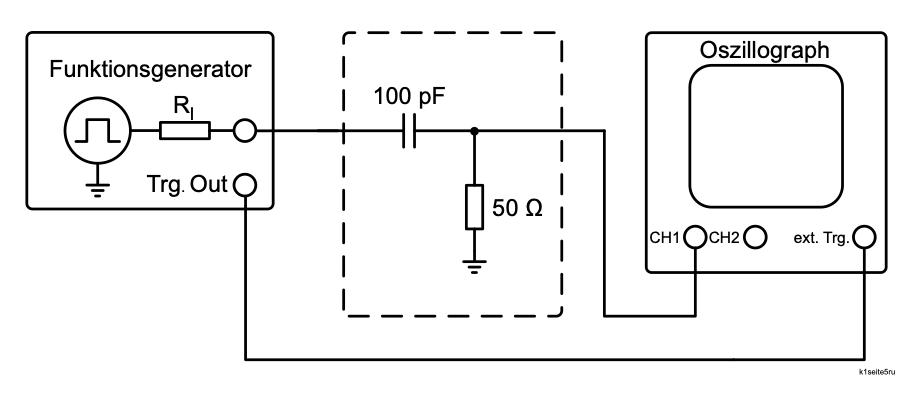
\includegraphics[width=0.8\textwidth]{Aufbau_1_1_Differenzierglied.png}
				\caption{Aufbau des Differenzierglieds \cite{anleitung}}
				\label{fig:aufbau_1_1_differenzierglied}
			\end{figure}
			Ein RC-Glied wird (ohne $\SI{2.2}{\kilo\ohm}$ Abschluss) zwischen einen Funktionsgenerator und einen Oszillographen geschaltet. Der Funktionsgenerator wird auf eine Frequenz von $\SI{200}{\kilo\hertz}$ eingestellt. Dann wird das Oszillogramm gezeichnet und dasselbe mit dem $\SI{2.2}{\kilo\ohm}$ Abschlusswiderstand wiederholt.
			%TODO: Messwerte & Auswertung
		\end{aufgabe}
		\begin{aufgabe}{Impulse auf Kabeln}
			
			\begin{figure}[h!]
				\centering
				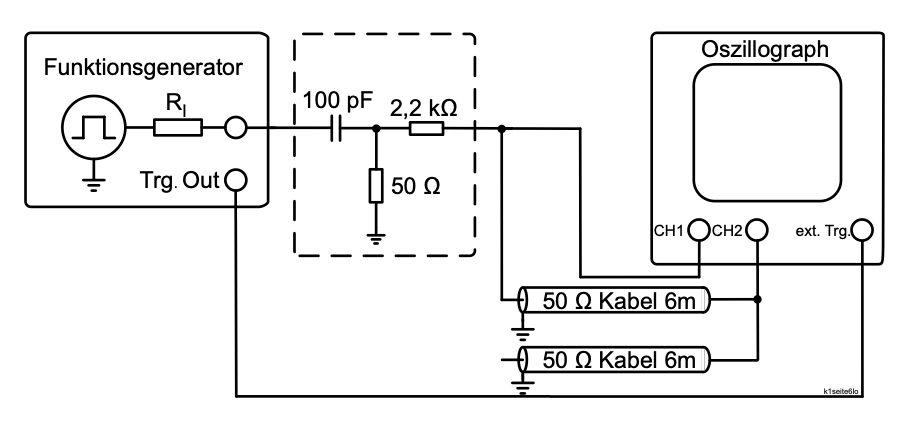
\includegraphics[width=0.8\textwidth]{Aufbau_1_2_Impulse_auf_Kabeln.png}
				\caption{Schaltplan für ein Kabel mit zwei offenen Enden \cite{anleitung}}
				\label{fig:aufbau_1_1_impulseAufKabeln}
			\end{figure}
			Jetzt sollen die Impulse auf einem an beiden Enden offenen Kabel untersucht werden. Dazu wird ein Funktionsgenerator, welcher im Rechteckmodus mit $\SI{100}{\kilo\hertz}$ betrieben wird, vor ein RC-Glied mit Abschluss, welches als Impulsgeber dient, geschaltet. Diese Impulse werden einerseits im CH1 des Oszillographen angezeigt, andererseits durch zwei hintereinandergeschaltete Kabel mit jeweils $\SI{50}{\ohm}$ Wellenwiderstand geschickt. Zwischen den beiden Kabeln wird der Oszillograph im CH2 geschaltet. Der Funktionsgenerator dient als externer Trigger für den Oszillographen, die beiden Kanäle werden mit derselben Empfindlichkeit betrieben.

			
		\end{aufgabe}
		\begin{aufgabe}{Leitungsabschluss, Verzögerungszeit}
			\begin{figure}[h!]
				\centering
				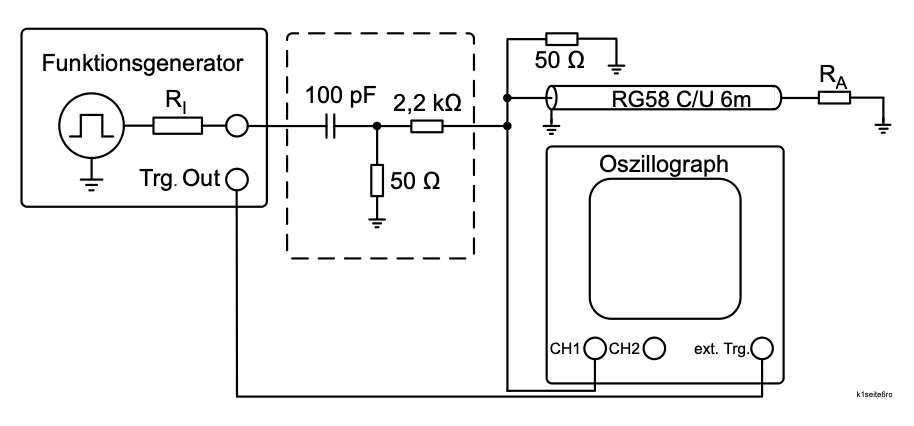
\includegraphics[width=0.8\textwidth]{Aufbau_1_3_Leitungsabschluss.png}
				\caption{Schaltplan für ein Kabel mit einem offenen und einem geschlossenen Ende \cite{anleitung}}
				\label{fig:aufbau_1_3_leitungsabschluss}
			\end{figure}
			Nun wird die Auswirkung unterschiedlicher Leitungsabschlüsse auf die Impulse untersucht. Dazu wird weiterhin extern getriggert, der Impulsgenerator wird auch an CH1 angeschlossen. Statt der beiden Kabel wird jetzt mittels eines T-Stücks ein Verzögerungskabel mit $\SI{50}{\ohm}$ Wellenwiderstand und $\SI{6}{\meter}$ Länge verwendet, welches am anderen Ende mit einem Widerstand $R_\mathrm{A} = \SI{50}{\ohm}$ abgeschlossen ist. Es für jede der folgenden Anordnungen mit und ohne einem zusätzlichen Widerstand von $\SI{50}{\ohm}$ parallel zum Kabel gemessen:
			\begin{enumerate}[(a)]
				\item Offenes Ende
				\item Offenes Ende im Detail ($\times 10$)
				\item Kurzgeschlossenes Ende
				\item Kurzgeschlossenes Ende bei verschiedenen Frequenzen (Zeitablenktung von $\SI{0.2}{\micro\second\per\centi\meter}$)
			\end{enumerate}
		\end{aufgabe}
		\begin{aufgabe}{Klippkabel, Dämpfung}
			\begin{figure}[h!]
				\centering
				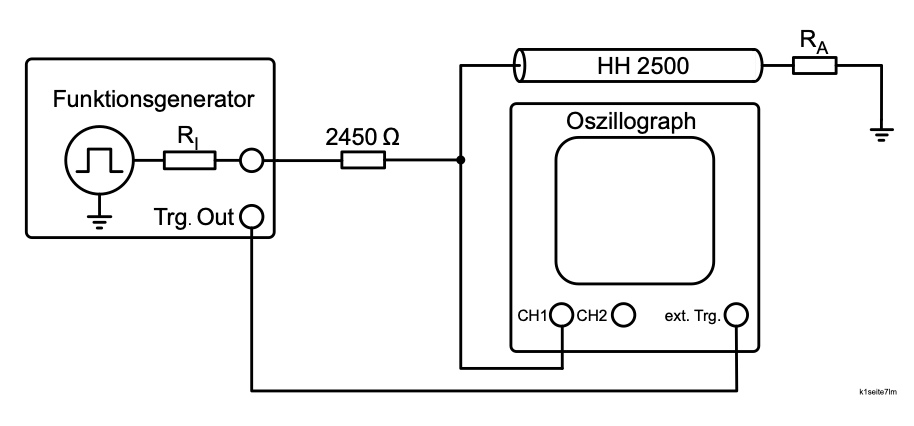
\includegraphics[width=0.8\textwidth]{Aufbau_1_4_Klippkabel.png}
				\caption{Schaltplan für ein Klippkabel \cite{anleitung}}
				\label{fig:aufbau_1_4_klippkabel}
			\end{figure}
			Zuletzt wird das Verzögerungskabel mit einem kürzeren, sogenannten Klippkabel, mit $\SI{0.7}{\meter}$ Länge ersetzt. Anstatt des Differenzierglieds wird ein Widerstand von $\SI{2450}{\ohm}$ eingebaut, der Widerstand vor dem Kabel wird entfernt. Der Funktionsgenerator wird auf eine Frequenz zwischen $\SI{10}{\kilo\hertz}$ und $\SI{80}{\kilo\hertz}$ eingestellt. Die Schaltverbindungen erfolgen mit $\SI{50}{\ohm}$ Koaxialkabeln. Dann wird unter den folgenden Umständen am Oszillographen gemessen:
			\begin{enumerate}[(a)]
				\item Klippkabel mit $\SI{50}{\ohm}$ Abschluss, d.h. offen
				\item Klippkabel kurzgeschlossen
				\item Klippkabel kurzgeschlossen mit variierter Frequenz
				\item $\SI{2}{\meter}$ Klippkabel kurzgeschlossen 
			\end{enumerate}
		\end{aufgabe}
		
		%TODO Aufbau/Schaltskizze (beschrieben in wenigen Worten)
		%TODO Versuchsdurchführung: Messgrößen, unabh. Parameter, Messmethode, Einheiten, Genauigkeit, wie oft
		%TODO Abgezeichnetes Messprotokoll vorhanden?

		%TODO Auswertung (in Worten & Formeln)
		%TODO Formeln symbolisch und numerisch
		%TODO Runden
		%TODO Grafiken & Diagramme: Überschrift, Messwerte mit Fehlerbalken, (nur) gefittete Kurven, Achsenbeschriftung
		%TODO Fehlerrechnung und -diskussion
		%TODO Jede Tabelle eine Formel
	\section{Fazit}
		%TODO Vollständiger Satz fürs Endergebnis
		%TODO Messergebnisse bewerten und evtl. mit Literaturwerten vergleichen
		%TODO Untersuchung Fehlerquellen (statistisch, systematisch, blödsinnig)
	\printbibliography
\end{document}
